% !TeX root = ../main.tex

\chapter{EPICS环境下基于POWERLINK的分布式IO系统}

在粒子加速器控制领域,EPICS是目前国际上应用最广泛的控制系统开发工具包,而开源实时以太网POWERLINK则广泛应用于工业控制领域,将POWERLINK和EPICS结合起来,可提高通信的实时性,拓宽EPICS的应用范围。我们基于FPGA开发了支持千兆POWERLINK通信协议的控制器并开发了相关的EPICS设备驱动程序,提出了两套EPICS环境下基于POWERLINK的分布式I/O系统方案,第一套方案的主站采用PC实现,我们称为主站PC方案;第二套方案是在主站PC方案基础上的升级版本,主站从站均基于FPGA实现,我们称之为全站FPGA方案。本章将分别介绍两套方案的系统架构设计、软硬件设计与开发,并分别搭建了相应的测试系统。最后,基于两套测试系统的具体情况,我们进一步完善了理论计算方法,并验证了仿真建模方法的可行性。

\section{主站PC方案的系统设计与开发}
\label{section:主站PC方案的系统设计与开发}

\subsection{系统架构设计}
\label{subsection:主站PC方案的系统架构设计}

主站PC方案的系统架构如~\ref{fig:design1-arch}图所示。

\begin{figure}[!htb]
  \centering
  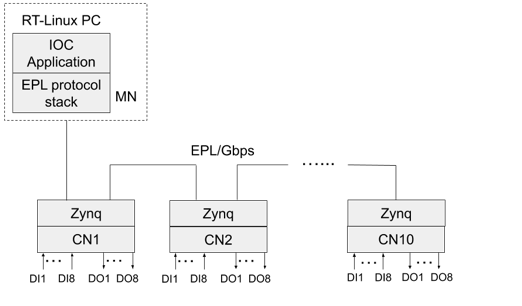
\includegraphics[width=0.7\textwidth]{design1-arch.png}
  \caption{主站PC方案系统硬件架构图}
  \label{fig:design1-arch}
\end{figure}

系统的网络拓扑为菊花链结构。该系统中有1个主站(MN)和10个从站(CN)组成,所有站点按照站点号从小到大的顺序依次连接,站点之间的通信基于千兆POWERLINK。主站是运行RT-Linux操作系统的PC,openPWERLINK程序和IOC应用程序也在运行在此PC上,其中openPOWERLINK工作在内核空间。从站是基于FPGA的控制器,支持千兆POWERLINK通信和集线器(HUB)功能。每个从站控制器都有多个DI和DO通道,可用于信号采集和输出\cite{xksun-2019}。

\subsection{主站程序的开发}

主站的软件架构如图~\ref{fig:design1-driver-arch}所示,由openPOWERLINK主站程序和IOC应用程序组成。IOC应用程序通过与openPOWERLINK主站程序建立通信,以监控POWERLINK网络中各节点的状态,所以IOC与POWERLINK主站之间的通讯实时性要求并不高。本方案中openPOWERLINK和IOC作为两个应用程序运行在同一台PC上,我们采用基于进程间Socket(IPC Socket)的通信方式来实现IOC应用程序与POWERLINK主站程序的通信。

\begin{figure}[!htb]
  \centering
  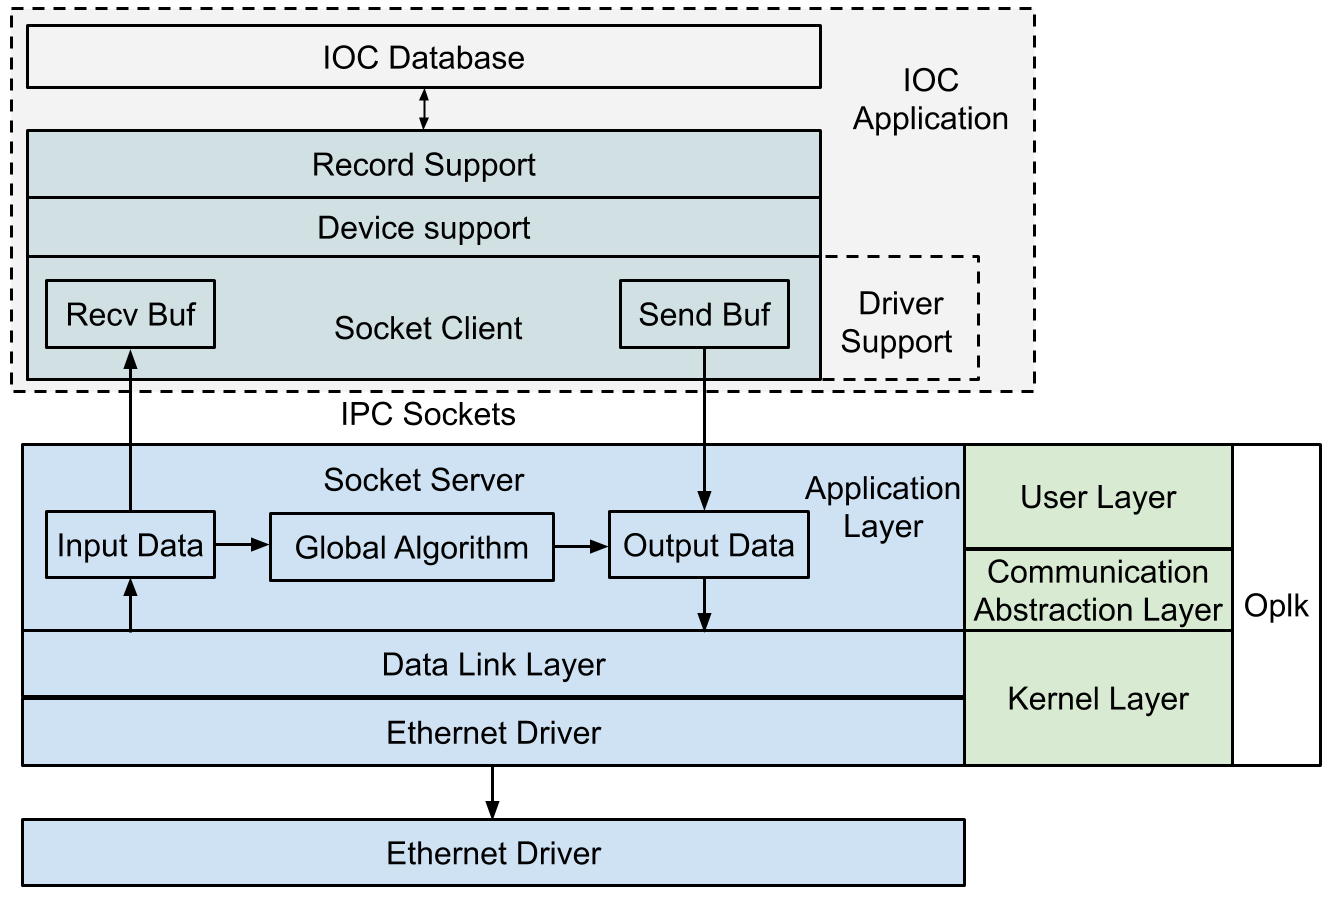
\includegraphics[width=0.7\textwidth]{design1-driver-arch.png}
  \caption{主站的软件架构图}
  \label{fig:design1-driver-arch}
\end{figure}

openPOWERLINK通过“Data Link Layer”收集各从站的DI信号,这些信号被发送到“Application Layer”中名为“Input Data”缓存区。同时作为Socket服务端,“Application Layer”会将“Input Data”缓存区中的数据传输到IOC应用程序。“Application Layer”中名为“Output Data”的缓存区用于接收来自IOC应用程序的控制参数等命令,并向下将控制参数发送到相应的从站。IOC应用程序通过EPICS驱动程序读取主站的数据,并转换为EPICS IOC中各种记录(Record)。驱动程序由“Driver Support”和“Device Support”组成。作为Socket客户端,“Driver support”中有两个缓存区,用于存储与openPOWERLINK程序交换的数据。在这些缓存区中,“Recv Buf”缓存区用于接收来自openPOWERLINK程序的数据,“Send Buf”缓存区用于存储发送至openPOWERLINK程序的控制参数。“Record Support”调用“Device Support”,将两个缓存区中的数据转化成EPICS中的记录,目前“Device Support”支持标准的EPICS DI和DO记录。

\subsection{从站控制器的设计与开发}
\label{subsection:前端控制器的设计与开发}
FPGA平台具有较高的实时性和灵活性,是实现POWERLINK协议较为理想的平台,也是目前普遍采用的方式。基于FPGA实现POWERLINK的方案有两种,软核方案是在FPGA中通过软核的形式来运行openPOWERLINK程序,HDL方案是采用纯硬件描述语言Verilog HDL来实现POWERLINK的协议栈。具体来说,HDL方案可以采用POWERLINK协议分离的方式来实现,数据链路层、物理层基于FPGA来实现,应用层基于ARM处理器来实现。这种设计既可以通过FPGA来达到较高的硬实时性,又可以利用ARM处理器来兼容各种应用层协议。

软核方案的技术细节和性能测试已在第~\ref{subsection:基于FPGA实现POWERLINK协议}节中详细介绍,对比软核方案,HDL方案有以下特点和性能优势:

(1) 采用硬件语言Verilog HDL来实现,无需软核,无需外扩RAM,即可以达到硬实时的性能。

(2) 实时性高,最短通信周期可以到达到几十$\mu$s,抖动可以达到数十ns。若采用MCU软核的方式,很难达到这样的性能指标。

(3) 对比第~\ref{subsection:基于FPGA实现POWERLINK协议}节中软核方案的通信过程,HDL方案使用硬件加速,在FPGA中实现自动回复功能。当PReq数据帧进入到FPGA中的MAC时,MAC会将准备好的上一周期的PRes数据快速发送到网络上。当使用了自动回复功能后,PReq数据帧和PRes数据帧之间的时间间隔可以达到几个$\mu$s,从而缩短通信周期,提高实时性。

(4) 兼容不同的应用层,虽然标准POWERLINK协议的应用层为CANopen,但是不同行业有不同的标准和习惯。采用此方案,可以仅使用Verilog HDL实现的数据链路层,而自定义应用层的协议。

(5) 兼容不同的物理层硬件,在保持数据链路层一致的情况下,此方案可以用于百兆、千兆以太网。


\subsubsection{硬件介绍}

从站控制器采用Xilinux Zynq-7000型号的芯片来实现POWERLINK协议,该芯片的结构如图~\ref{fig:Zynq-arch}所示。Zynq-7000器件在硬件上配备了双核ARM Cortex-A9处理器,该处理器与基于28nm Artix-7的可编程逻辑集成,在软件上兼具ARM处理器的软件可编程性与FPGA的硬件可编程性。由于其高度的灵活性和较小的硬件占用空间,Zynq是自动化项目中小型高性能设备的理想平台\cite{zynq-7000}。我们可以利用Zynq芯片的ARM处理器实现POWERLINK协议的应用层,利用FPGA实现POWERLINK协议的数据链路层和物理层,从而达到硬实时的性能。

\begin{figure}[!htb]
	\centering
	\includegraphics[width=0.8\textwidth]{Zynq-arch.png}
	\caption{Xilinux Zynq-7000芯片的架构图}
	\label{fig:Zynq-arch}
\end{figure}

基于Zynq设计了由核心板和底板组成的控制器,核心板通过相应引脚与底板相连接,核心板的硬件架构如图~\ref{fig:zynq-core-board-arch}所示,底板的硬件架构如图~\ref{fig:zynq-floor-arch}所示。

核心板硬件系统的各部分为:

(1) 核心片:POWERLINK网络通信的核心部件,选用Xilinux Zynq-7000家族的芯片,具体型号为XC7Z020,逻辑单元数为85k。

(2) 外部存储:外部存储连接到ARM硬核上,包括512MB的DDR3、16MB的Qspi$\_$Flash、4GB的EMMC和TF$\_$CARD,用来提供POWERLINK程序的运行空间和存储空间。

(3) Reset$\&$WatchDog:外置看门狗计时器,用来复位程序。

(4) Gig$\_$Ethernet:千兆以太网PHY芯片,通过此以太网接口与EPICS IOC应用程序通信。

(5) JTAG接口:POWERLINK协议程序的下载和调试接口。

(6) Expansion IO:扩展IO引脚,用于连接底板。

\begin{figure}[!htb]
	\centering
	
\includegraphics[width=0.7\textwidth]{zynq-core-board-arch.png}
	\caption{基于Zynq的核心板硬件架构图}
	\label{fig:zynq-core-board-arch}
\end{figure}


底板硬件系统的各部分为:

(1) POWERLINK×2:用于POWERLINK通信的HUB的两个千兆以太网接口。

(2) GPIOs:提供DI、DO接口。

(3) 本地通讯接口:提供了RS232、RS484以及CAN本地通讯接口。

\begin{figure}[!htb]
	\centering
	
\includegraphics[width=0.7\textwidth]{zynq-floor-arch.png}
	\caption{基于Zynq的底板硬件架构图}
	\label{fig:zynq-floor-arch}
\end{figure}

图~\ref{fig:design1-board-photo}所示的是控制器电路板实物,可从照片中看出GPIO接口、两个POWERLINK网口。

\begin{figure}[!htb]
	\centering
	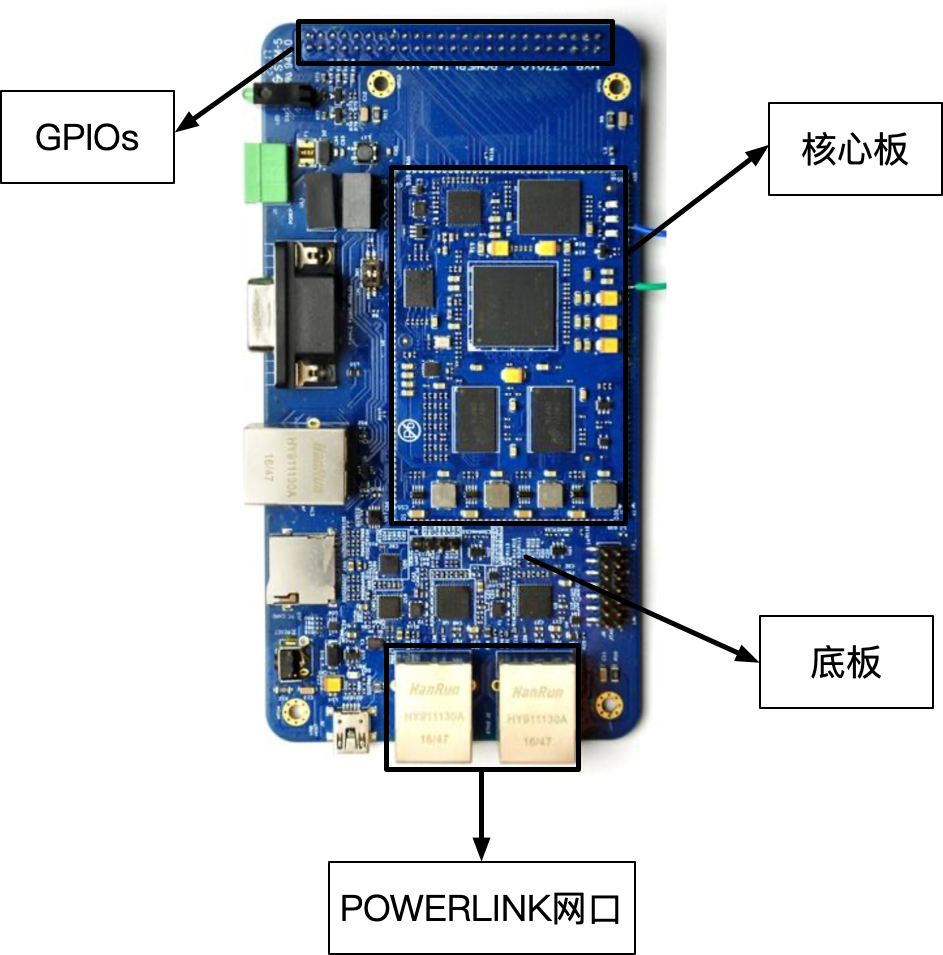
\includegraphics[width=0.6\textwidth]{design1-board-photo.png}
	\caption{控制器电路板照片}
	\label{fig:design1-board-photo}
\end{figure}

\subsubsection{软件设计}

基于Zynq的硬件架构,设计了如图~\ref{fig:design1-zynq-software}所示的从站软件架构。由三部分组成:基于ARM处理器的POWERLINK应用层、基于FPGA的POWERLINK数据链路层和物理层。

\begin{figure}[!htb]
  \centering
  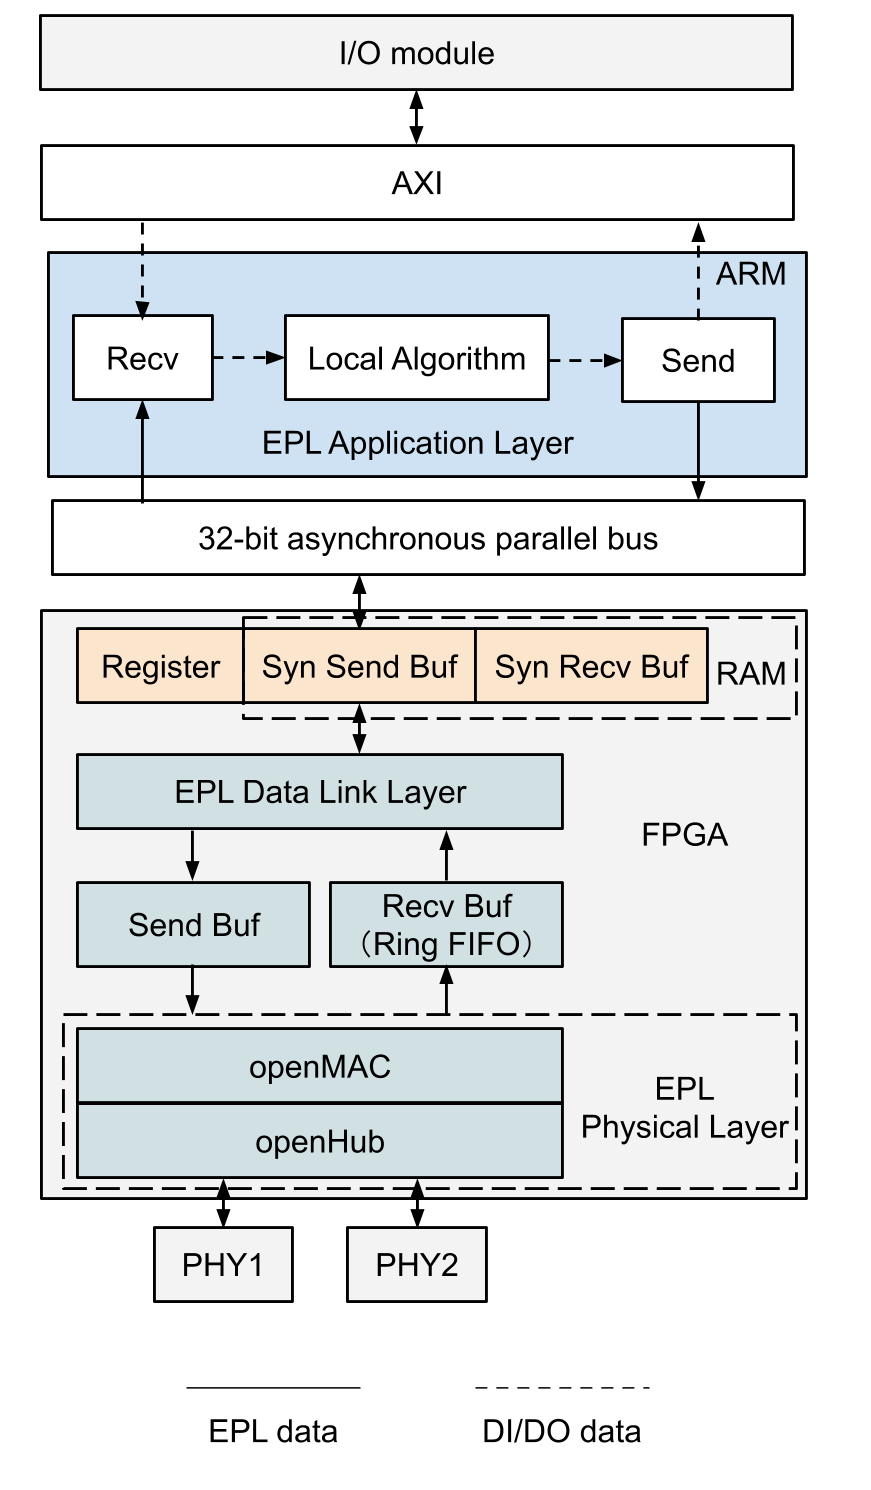
\includegraphics[width=0.6\textwidth]{design1-zynq-software.png}
  \caption{基于Zynq的控制器软件架构图}
  \label{fig:design1-zynq-software}
\end{figure}

\begin{itemize}

\item \textbf{物理层} \\ 
POWERLINK物理层采用Verilog HDL实现,由openHub和openMAC两部分组成。openMAC支持千兆以太网PHY芯片,双口openHUB可以以菊花链的形式来连接两个相邻的从站。 

\item \textbf{数据链路层} \\ 
POWERLINK的数据链路层状态机和NMT网络管理等采用Verilog HDL来实现。

\item \textbf{应用层} \\ 
POWERLINK协议的应用层基于ARM架构,采用C语言实现。除了可以使用标准POWERLINK的CANopen应用层以外,还支持其他任意的应用层。

\item \textbf{API接口} \\ 
应用层与数据链路层之间的接口为API接口。该接口采用寄存器和双口RAM实现,应用层通过32位并行总线来访问寄存器和双口RAM中的数据。

\end{itemize}

数据传输的流程和细节如下:

 (1) POWERLINK应用层通过32位并行总线将数据写入寄存器和“Syn Buf”缓存区,缓存区采用双口RAM实现,从而避免数据链路层和应用层同时对RAM操作造成的冲突。
 
 (2) 在数据链路层和应用层之间,有“Sync Recv Buf”和“Sync Send Buf”两个缓存区,分别用于保存数据链路层收到的同步数据和下个周期要发送的同步数据。同步数据是周期性传输的数据,在每个周期开始的时候,数据链路层都会给应用层一个同步中断信号,触发应用层的同步回调函数对“Sync Send Buf”和“Sync Recv Buf”两个缓存区中的数据进行读写操作。
 
 (3) 数据链路层组建要发送的数据包,并写入MAC层的“Send Buf”缓存区中,然后启动发送。发送完成后,通过寄存器的标志位来反馈发送是否正确。
 
 (4) MAC层接收到数据时,将其放到MAC层的“Recv Buf”缓存区中,该缓存区为环形,可以存放2个最大以太网的帧。当收到一个完整且正确的PReq数据帧,即该数据帧的目标节点号与本节点相同,则通知数据链路层进行处理,将数据帧的有效数据部分从MAC的“Recv Buf”拷贝到“Sync Recv Buf”中。如果接收到的数据有问题,则丢弃本帧数据,并将重新设置MAC的接收设置,为下一次接收做准备。当处理完毕后,通知MAC层释放接收缓冲区“Recv Buf”,用来保存后面的数据帧。

除了完成POWERLINK协议通信,从站还需要完成IO信号的采集、本地处理和输出。如图~\ref{fig:design1-zynq-software}所示,IO模块的数据存储在外部RAM中,应用层通过AXI总线来读写RAM中的IO数据,应用层的本地算法模块用来对IO数据进行本地处理。

\subsection{测试系统搭建}

为测试主站PC方案设计系统的实时性能,基于第~\ref{subsection:主站PC方案的系统架构设计}节设计的系统架构,我们搭建了相应的测试系统,以下将分别介绍系统的硬件组成和软件开发。

\subsubsection{测试系统的硬件组成} 

按照第~\ref{subsection:主站PC方案的系统架构设计}节设计的主站PC方案,我们搭建了如图~\ref{fig:prototype-mn-pc-photo}所示的测试系统。该系统由1台PC和10台FPGA控制器组成。EPICS IOC应用程序和openPOWERLINK主站程序运行在在同一台PC上,PC上安装了带有内核实时补丁3.10的Centos7系统。该PC的网卡型号为intel 82573,openPOWERLINK主站程序通过该网卡驱动,运行在在内核模式下。

\begin{figure}[!htb]
	\centering
	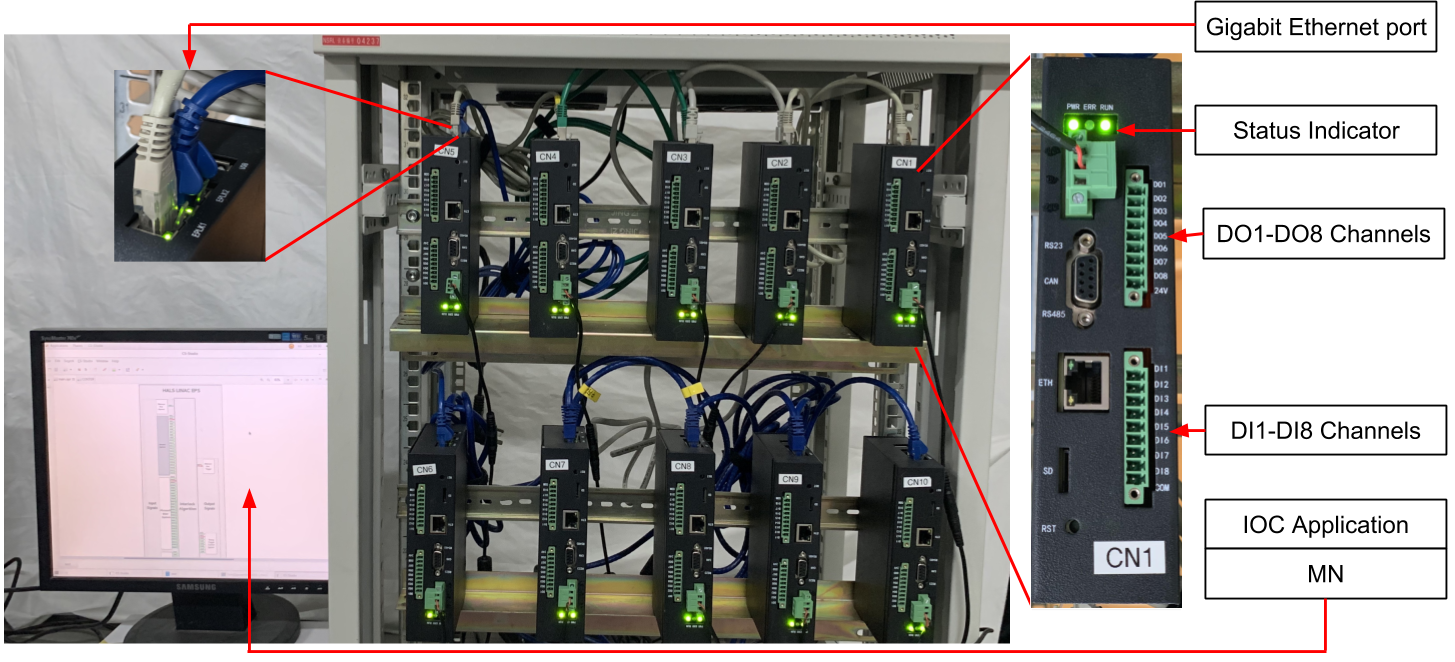
\includegraphics[width=\textwidth]{prototype-mn-pc-photo.png}
	\caption{主站PC方案的系统照片}
	\label{fig:prototype-mn-pc-photo}
\end{figure}


测试系统共有10个从站,每个从站都是基于Zynq的控制器。控制器对外提供了8个DI和8个DO通道,DI接口如图~\ref{fig:zynq-8di-interface}所示,公共端(COM0端口供DI输入使用,输入设备的地需要与此处共地形成回路;DO接口如图~\ref{fig:zynq-8do-interface}所示,为源型输出,24V输入端为DO输出负载所接的正24V电压。另外,2个千兆以太网端口用于连接相邻的从站,3个状态指示灯分别显示控制器的电源状态,错误状态和操作状态,灯亮表示状态正常。

\begin{figure}[!htb]
	\centering
	
\includegraphics[width=0.8\textwidth]{zynq-8di-interface.png}
	\caption{从站控制器DI接口}
	\label{fig:zynq-8di-interface}
\end{figure}

\begin{figure}[!htb]
	\centering
	
\includegraphics[width=0.8\textwidth]{zynq-8do-interface.png}
	\caption{从站控制器DO接口}
	\label{fig:zynq-8do-interface}
\end{figure}

\subsubsection{测试系统的软件开发}

\label{subsubsection:测试系统软件开发}

测试系统的软件开发包括主站程序和从站程序的开发。基于Zynq的从站控制器程序按照图~\ref{fig:design1-zynq-software}所示的软件架构开发,除了完成POWERLINK通信以外,在POWERLINK应用层加入了本地算法功能,从站控制器可以直接对DI信号进行处理,并输出DO信号。主站程序包括来EPICS IOC应用程序和openPOWERLINK主站程序,IOC应用程序的开发按照图~\ref{fig:design1-driver-arch}所示的软件架构展开,openPOWERLINK主站程序的应用层加入了全局算法功能,主站通过全局算法处理来自各从站控制器的DI信号,并通过相应的从站输出DO信号。openPOWERLINK主站应用层程序和Zynq控制器应用层程序类似,程序框架如下:
\begin{lstlisting}
while(1)
{ 
  //处理出来POWERLINK网络状态机跳转,网络配置等
  ret = oplk_process();

  //主站UDP Server通信程序
  udp_send_data((const char *) UDP_TX_Buffer, int data_len);
  udp_recieve_data(const char *frame, int data_len);

  //从站读写DI/DO和本地算法程序
  CHA_DI_read(u32 Input_Pin);
  local_process_data();
  FPGA_DO_write(u32 Output_Pin, u32 Data);
}

//同步回调函数,由SoC触发
void syncCb(void)
{
  //负责读写同步数据和主站全局算法程序
  pdou_copyRxPdoToPi();
  global_process_data();
  pdou_copyTxPdoFromPi();
}
\end{lstlisting}

程序主要由while循环程序和POWERLINK通信同步回调函数组成。while循环程序一直运行,用来处理POWERLINK异步事件、状态机跳转、网络配置等。对于主站我们在while循环程序里添加了UDP Server程序;对于从站,我们在while循环程序里添加了DI/DO读写和和本地算法程序。通信同步回调函数“synCb( )”由SoC触发,用于处理周期性同步数据,我们在此添加了全局算法程序。


\subsection{系统性能测试与分析}

主站PC方案中的IOC负责监控POWERLINK网络中各节点状态,并不直接参与POWERLINK通信,所以系统实时性能即是系统中POWERLINK网络部分的实时性能。我们对测试系统的POWERLINK网络进行了一系列性能测试,其中包括通信周期、本地响应时间、全局响应时间和主站响应时间,下面将详细介绍测试细节和测试结果。

\subsubsection{系统通信周期测试}

\label{subsection:主站PC方案系统通信周期测试}

通信周期是衡量实时系统性能的重要参数,短时间周期内持续稳定运行对于实时性系统至关重要。我们使用openCONFIGURATOR网络组态工具来配置不同的POWERLINK通信周期,利用ProfiShark 1G Ethernet Troubleshooter以太网诊断工具来测试系统在不同通信周期下的运行情况,从而确定系统最短通信周期。ProfiShark 1G是一款专用于千兆以太网监测的故障诊断仪,硬件时间戳仅为8ns,可以抓取高实时性的POWERLINK通信数据,将抓包结果输出为可被Wireshark解析的pcap格式文件。

我们对主站PC方案系统进行了通信周期测试,测试结果如下:图~\ref{fig:design1-cycle-time-test}所示的是主站PC方案系统的数据帧抓取结果,通信周期可根据两个连续SoC帧之间的时间隔计算得出的,如图~\ref{fig:design1-cycle-time-test}所示。我们抓取来超过12k个连续的POWERLINK帧,并将通信周期的概率密度分布绘制在图~\ref{fig:design1-cycle-time-density}中。图~\ref{fig:design1-cycle-time-density}表明,大多数情况下的通信周期都非常接近系统的通信周期设定值275$\mu$s,通信周期周期的最大偏移约为12$\mu$s。

\begin{figure}[!htb]
  \centering
  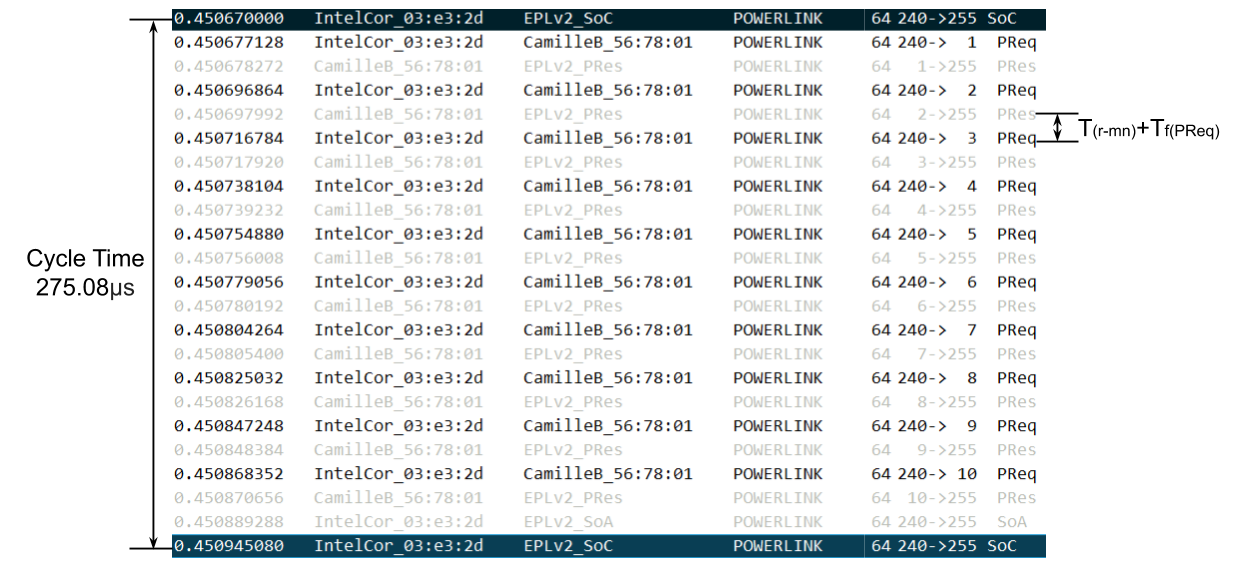
\includegraphics[width=0.85\textwidth]{design1-cycle-time-test.png}
  \caption{测试系统的POWERLINK数据帧抓取结果}
  \label{fig:design1-cycle-time-test}
\end{figure}

\begin{figure}[!htb]
  \centering
  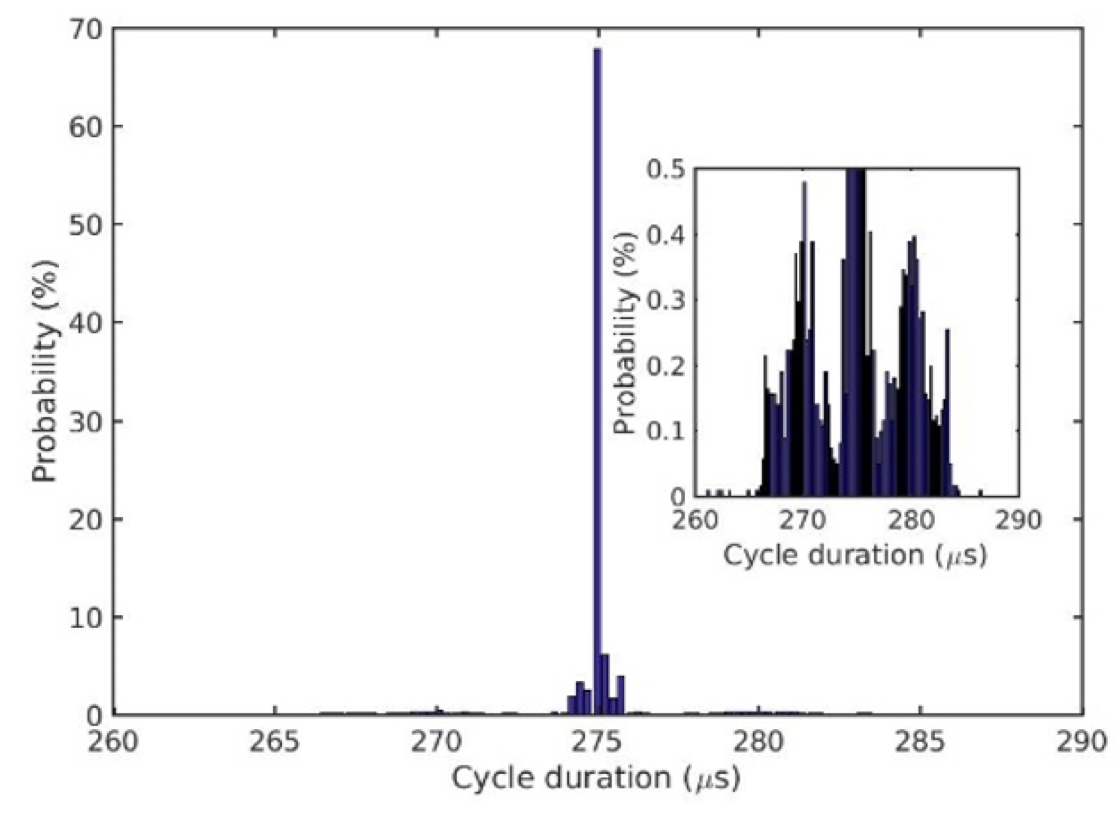
\includegraphics[width=0.85\textwidth]{design1-cycle-time-density.png}
  \caption{测试系统的POWERLINK通信周期概率密度分布}
  \label{fig:design1-cycle-time-density}
\end{figure}


\subsubsection{响应时间测试}
响应时间是指DI信号到达系统与系统输出DO信号之间的时间间隔,是衡量系统实时性能的重要参数。我们测试了本地响应和全局响应两种参数,本地响应指是从站本身对于DI信号直接做出的响应;全局响应是指DI信号经过POWERLINK网络传输,被主站处理之后,系统做出的响应。

首先对从站控制器进行本地响应时间的测量,本地响应的过程如下:

(1) 从站的GPIO读取输入信号,并将输入值以二进制形式存储在外部RAM中;

(2) 运行在ARM上的应用层程序通过AXI总线读取并处理RAM中的输入数据;

(3) 处理结果通过AXI总线写入相应的外部RAM中并通过GPIO输出信号。

我们将1号从站控制器的输入和输出信号连接到示波器上,以输入和输出信号的上升沿时间差来表示本地响应时间。测试结果如图~\ref{fig:design1-local-response-time}所示,Ch1(黑线)代表1号从站控制器的输入信号; Ch2(青色线)代表1号从站控制器的输出信号,响应时间约为400$\mu$s。这个时间延迟包括从站控制器输入/输出接口电路中的光电耦合器的延时和ARM读取处理数据的时间。由于ARM的时钟频率为125MHz,AXI总线传输的数据宽度为32bit,所以运行在ARM上的应用层程序通过AXI总线读取处理数据的时间不到1$\mu$s,所以本地响应时间主要是光电耦合器导致的延时。

\begin{figure}[!htb]
	\centering
	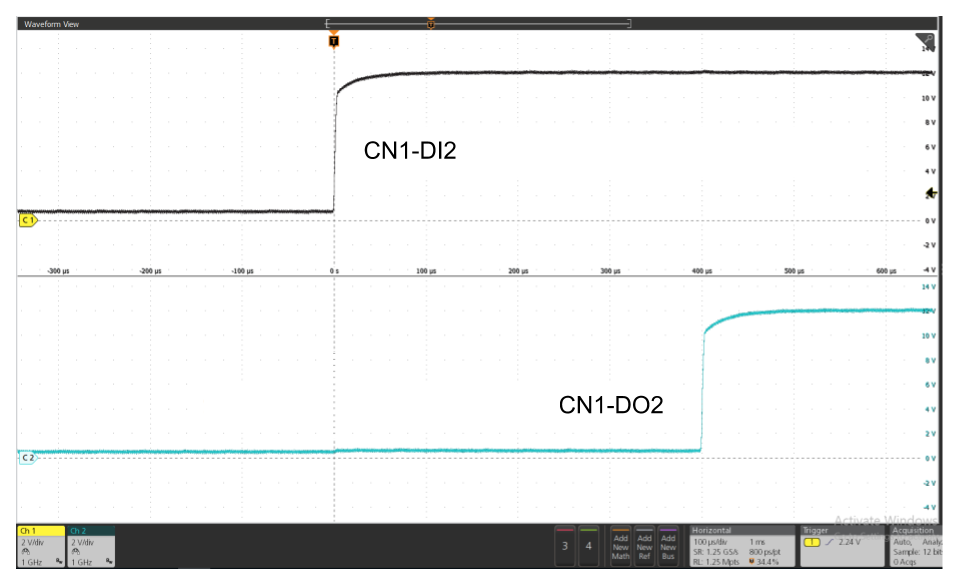
\includegraphics[width=\textwidth]{design1-local-response-time.png}
	\caption{本地响应时间测试结果}
	\label{fig:design1-local-response-time}
\end{figure}

\begin{figure}[!htb]
  \centering
  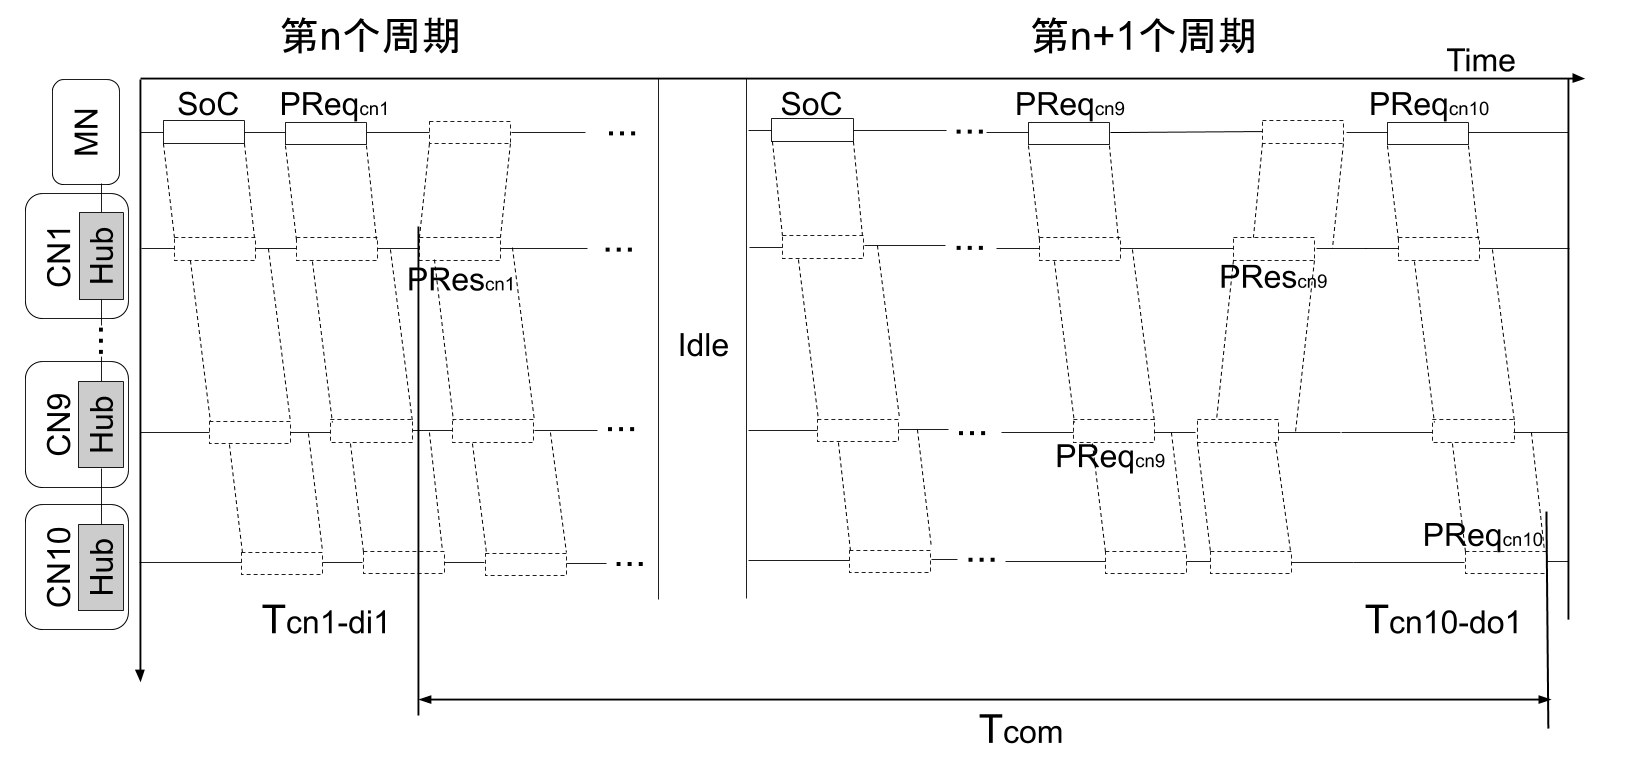
\includegraphics[width=\textwidth]{design1-response-process.png}
  \caption{全局响应过程}
  \label{fig:design1-response-process}
\end{figure}

全局响应时间($T_{global-response}$)由POWERLINK网络通信时间($T_{com}$)和从站处理输入/输出信号的时间($T_{CN-process}$)组成,可以用公式~\ref{equation15}来表示。POWERLINK网络通信时间包括用于封装和解封装数据帧的时间、主站处理数据的时间、电缆中数据传输的时间以及HUB中的时间延迟。从站处理输入/输出信号的时间可以用公式~\ref{equation16}来表示,包括了光耦合器的延时($T_{coupler}$)和输入信号等待进入POWERLINK通信的时间$T_{wait}$)。

\begin{equation}
\label{equation15}
T_{global-response}=T_{com}+T_{CN-process}
\end{equation}

\begin{equation}
\label{equation16}
T_{CN-process}=T_{coupler}+T_{wait}
\end{equation}

在全局响应时间的测试中,我们设计了如图~\ref{fig:design1-response-process}所示的响应过程。在第n个周期,1号从站的输入信号通过PRes数据帧进入POWERLINK网络,$T_{cn1-di1}$为1号从站接收到输入信号的时刻,该信号经过主站处理之后,处理结果在第n+1个周期通过PReq数据帧从10号从站输出,$T_{cn10-do1}$为10号从站输出信号的时刻。该响应过程经历两个连续周期,$T_{com}$是此过程的通信时间。根据POWERLINK通信顺序,10号从站是通信周期中的最后一个参与通信的。因此,$T_{com}$也是该系统全局响应的最长通信时间。如图~\ref{fig:design1-cycle-time-test}所示,可以使用ProfiShark 1G以太网分析仪捕获数据帧来计算$T_{com}$,大约为457$\mu$s。示波器测得的总响应时间如图~\ref{fig:design1-response-time-result}所示,Ch1(黑线)代表1号从站控制器的输入信号; Ch3(红色线)代表10号从站控制器的输出信号,响应时间约为870$\mu$s。考虑到在本地响应过程光电耦合器引起的延迟时间($T_{coupler}$)约为400$\mu$s,输入信号在“Sync Send Buf”缓存区等待被发送的时间($T_{wait}$),输入信号等待进入POWERLINK通信的时间($T_{wait}$)约为21$\mu$s。

\begin{figure}[!htb]
  \centering
  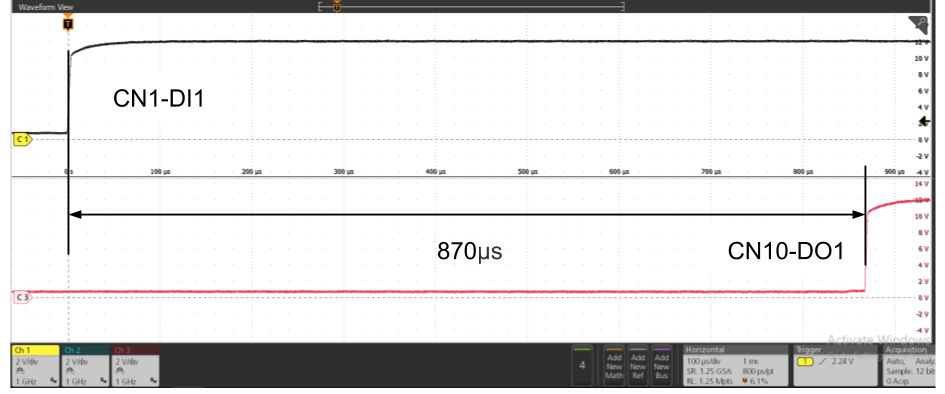
\includegraphics[width=\textwidth]{design1-response-time-result.png}
  \caption{全局响应时间测试结果}
  \label{fig:design1-response-time-result}
\end{figure}

主站的响应时间是指当主站收到来自从站的PRes数据帧到回复PReq数据帧的时间。主站在每个从站通信时隙中都需要响应PReq数据帧,所以主站响应时间直接影响系统的通信周期,进而影响到系统响应时间,而且随着从站数量的增加,影响会加大。主站响应时间与设备类型有关,主站PC方案的主站采用的是基于x86运行Linux的PC。如图~\ref{fig:design1-cycle-time-test}所示,相邻PRes数据帧和PReq数据帧之间时间差为主站响应时间($T_{r-mn}$)和PReq数据帧的传输时间($T_{F(PReq)}$)之和。PReq数据帧长度为64Byte,采用千兆以太网传输,则$T_{F(PReq)}$为0.640$\mu$s。由此计算得到主站PC方案运行Linux PC的主站平均响应时间约为16.168$\mu$s。

\subsubsection{测试小结}
本节对主站PC方案的测试系统进行了包括通信周期、系统响应时间和主站响应时间的性能测试,根据测试结果,总结如下:

(1) 主站PC方案的测试系统在10节点情况下,可以在275$\mu$s通信周期下运行,系统全局响应时间为870$\mu$s。

(2) 测试系统的本地响应时间为400$\mu$s,此延时较大,主要是从站输入/输出接口电路中的光耦合器的延时造成的。

(3) 从站控制器的DI/DO通道数量较少,难满足真实的工程应用需求,可采用数据选择器来扩展DI/DO通道数量。

(4) 主站是运行Linux系统的PC,较之FPGA,PC的响应时间较慢,响应时间约为16.168$\mu$s。主站的openPOWERLINK程序运行在内核空间下,对以太网网卡类型依赖严重,需要针对不同的网卡类型开发相应的驱动程序,程序可移植性差。主站可采用Zynq控制器来实现,提高反应时间,缩短通信周期。

\section{全站FPGA方案的系统设计与开发}
\label{section:全站FPGA方案的系统设计与开发}

\subsection{系统架构设计}
\label{subsection:全站FPGA方案系统架构设计}
全站FPGA方案的系统架构如图~\ref{fig:design2-arch}所示,由1个主站和5个从站组成,网络拓扑为线型拓扑结构,所有站点均按站点号从小到大顺序依次连接,站点之间的通信基于千兆 POWERLINK。主站是基于Zynq的控制器,IOC应用程序运行在PC上,IOC应用程序通过千兆以太网与主站通信。从站是基于Zynq的控制器,支持千兆POWERLINK通信和集线器(HUB)功能。每个从站控制器都有128路DI和16路DO通道,用于信号采集和输出。

\begin{figure}[htbp]
  \centering
  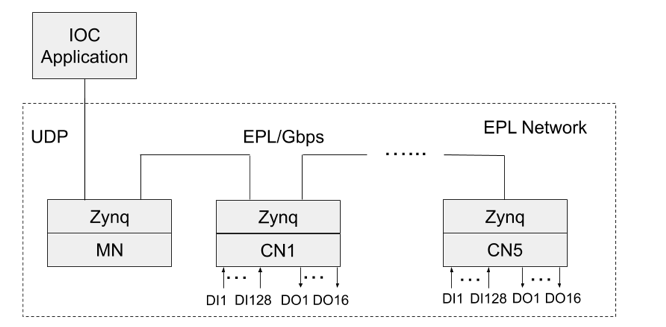
\includegraphics[width=\textwidth]{design2-arch.png}
  \caption{全站FPGA方案的系统硬件架构图}
  \label{fig:design2-arch}
\end{figure}

\subsection{从站控制器的设计与开发}

\subsubsection{硬件介绍}

\begin{figure}[htbp]
  \centering
  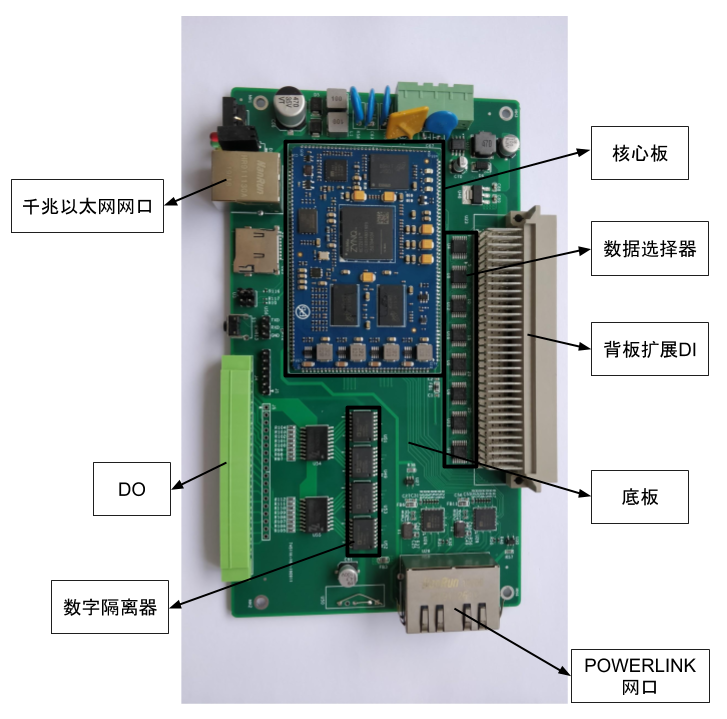
\includegraphics[width=0.7\textwidth]{design2-zynq-board-photo.png}
  \caption{从站控制器电路板照片}
  \label{fig:design2-zynq-board-photo}
\end{figure}

\begin{figure}[htbp]
  \centering
  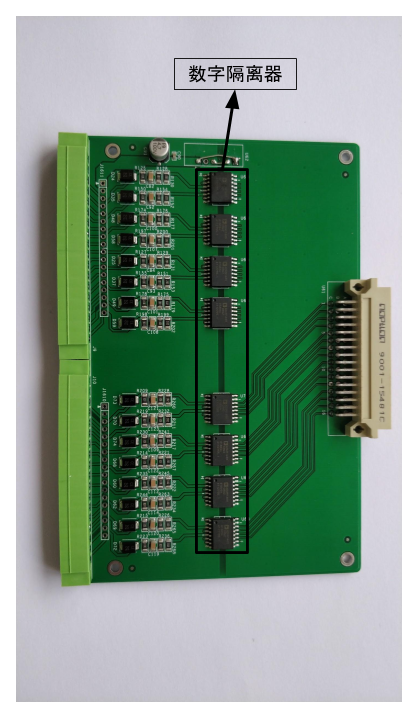
\includegraphics[width=0.4\textwidth]{di-expansion-board.png}
  \caption{从站控制器DI扩展板照片}
  \label{fig:di-expansion-board}
\end{figure}

全站FPGA方案中的主站控制器的硬件选型与设计和主站PC方案从站控制器基本相同,不同的是主站控制器增加了一个千兆以太网口,用于与IOC应用程序通信,具体可以参见第~\ref{subsection:前端控制器的设计与开发}节中硬件介绍部分,在此不再赘述。从站控制器采用主板、DI扩展板和背板相结合的方式来实现,主板和DI扩展板为独立板卡,背板为母板,主板和DI扩展板均插接与背板上。图~\ref{fig:design2-zynq-board-photo}所示的是全站FPGA方案从站控制器主板实物,主板由核心板和底板组成,硬件设计与主站PC方案的从站控制器基本相同。不同的是,全站FPGA方案主板增加了背板扩展DI接口用于连接背板,主板输出接口电路采用了高速数字隔离器,数字隔离器的型号是ADuM1400。主板采用4选1数据选择器来扩展DI通道数量,数据选择器型号为SN54HC153。图~\ref{fig:di-expansion-board}所示的是DI扩展板实物,DI扩展板输入接口电路同样采用了ADuM1400数字隔离器,4块DI扩展板共提供了128路DI通道,这种设计更具实际应用价值。


\subsubsection{软件设计}

从站控制器的软件架构如图~\ref{fig:design2-zynq-software},由三部分组成:基于ARM处理器的POWERLINK应用层、基于FPGA的POWERLINK数据链路层和物理层。实现方式与主站PC方案基本相同,具体可以参见第~\ref{subsection:前端控制器的设计与开发}节中软件设计部分,在此不再赘述。不同的是,IO模块的数据直接存储在FPGA内部双口RAM中,较之主站PC方案,这种设计减少了读写的延时,使得数据读写速度更快,运行在ARM上的应用层程序通过32位并行总线来读写RAM中的数据。

\begin{figure}[htbp]
  \centering
  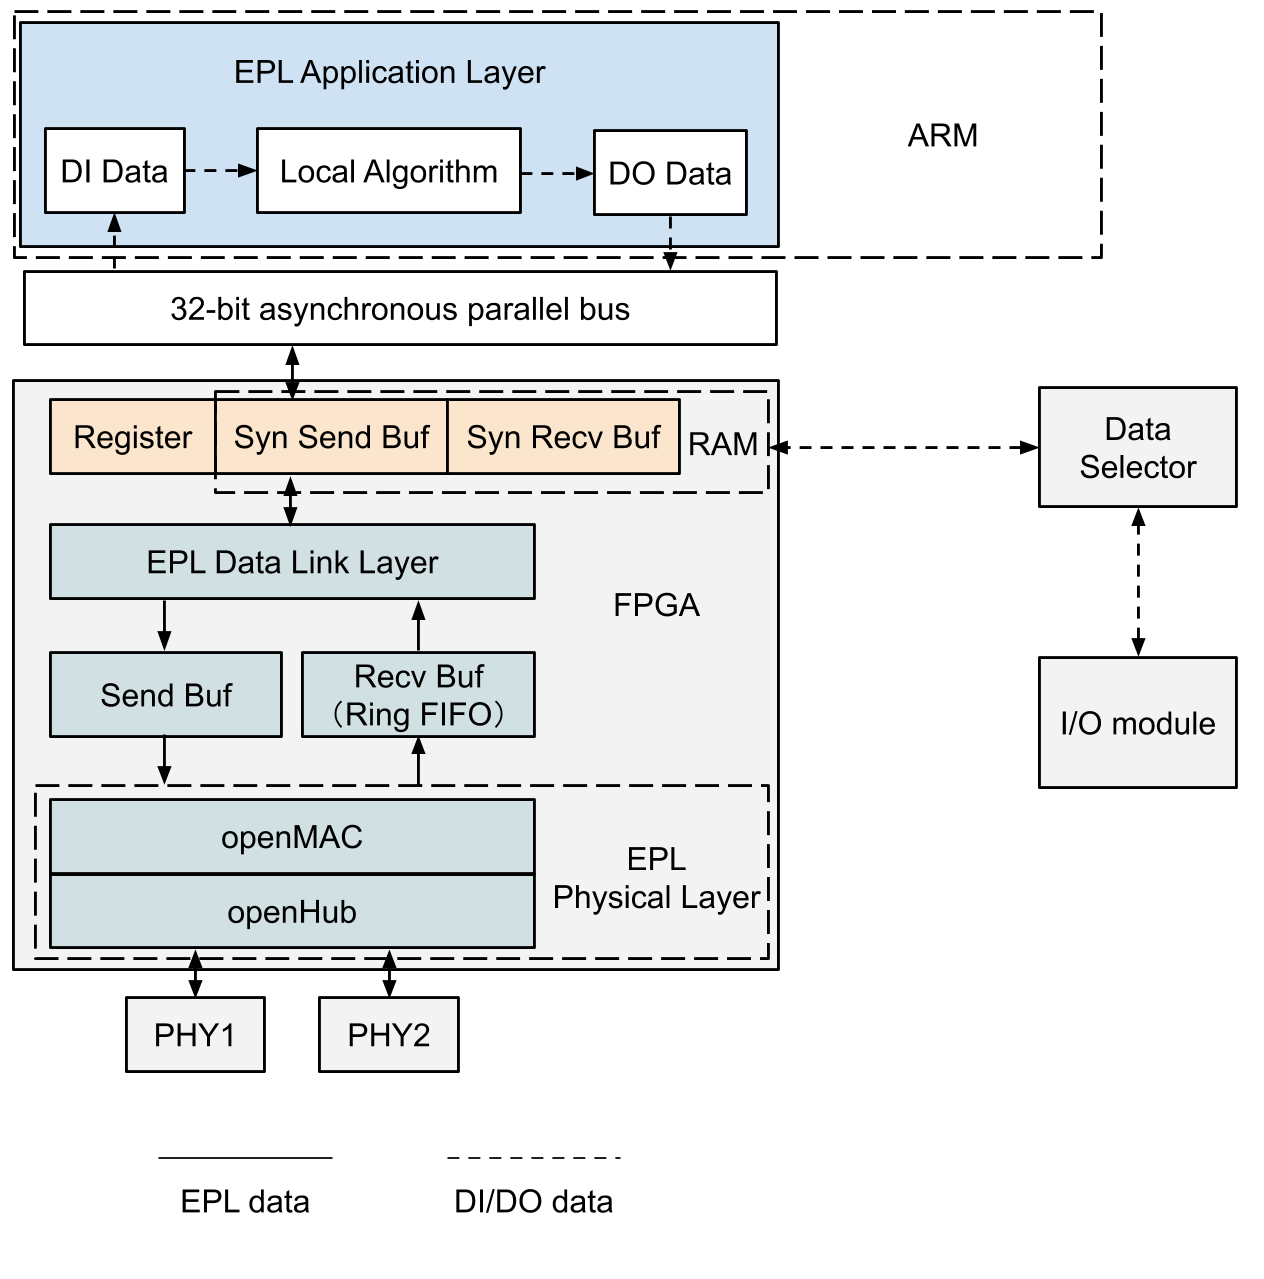
\includegraphics[width=0.8\textwidth]{design2-zynq-software.png}
  \caption{基于Zynq的从站控制器软件架构图}
  \label{fig:design2-zynq-software}
\end{figure}

主站控制器的软件架构与从站类似,主站应用层保持数据链路层和物理层不变的同时,在应用层添加了UDP客户端通信模块和全局算法模块,如图~\ref{fig:design2-driver-arch}所示的MN部分。

\subsection{EPICS设备驱动程序的开发}

IOC应用程序运行在Linux PC上,主站是基于Zynq的控制器,我们采用基于UDP Socket的通信方式来实现二者之间的通信。具体实现方式如图~\ref{fig:design2-driver-arch}所示,主站(MN)的“Data Link Layer”收集各从站的DI信号,这些信号被发送到“Application Layer”中名为“Input Data”缓存区中。作为UDP客户端,“Application Layer”会将“Input Data”缓存区中的数据传输到IOC应用程序。“Application Layer”中名为“Output Data”的缓存区用于接收来自IOC应用程序的控制参数等命令,并向下将控制参数发送到相应的从站。“Application Layer”加入了全局算法功能,主站通过全局算法处理来自各从站控制器的DI信号,并通过相应的从站输出DO信号。

\begin{figure}[htbp]
  \centering
  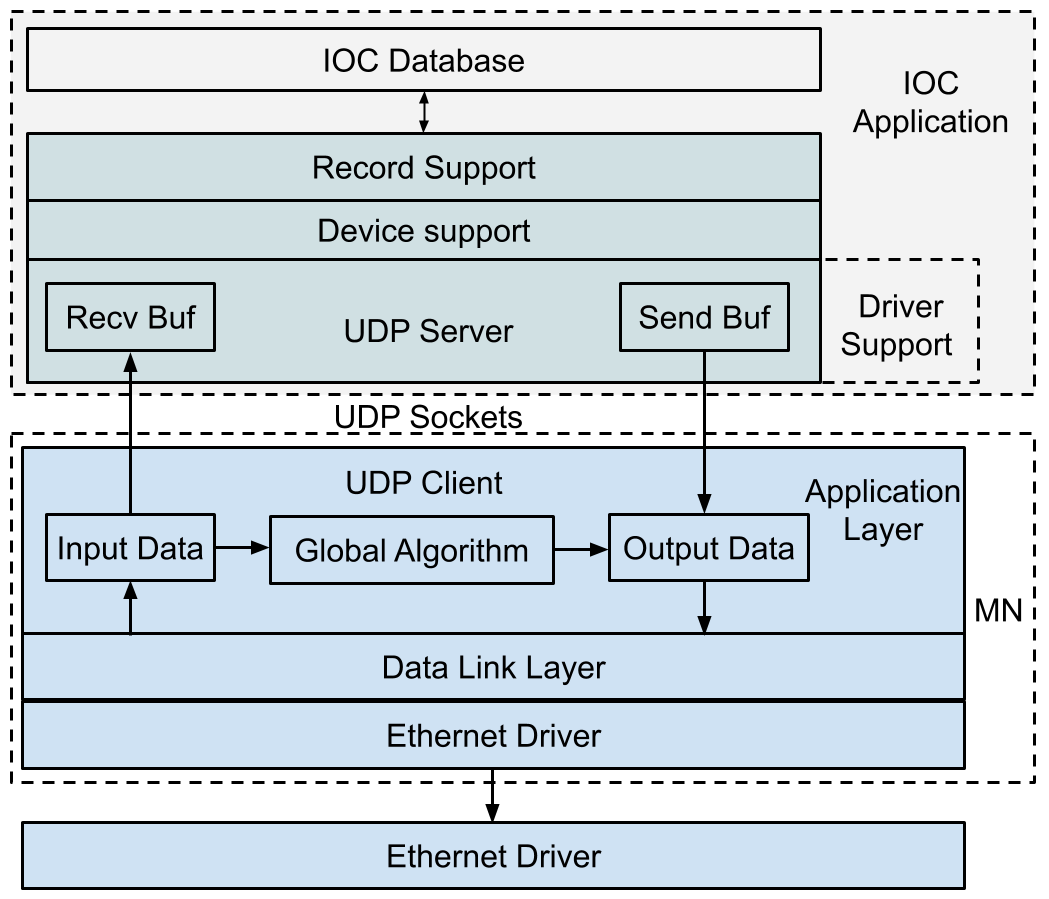
\includegraphics[width=0.8\textwidth]{design2-driver-arch.png}
  \caption{EPICS设备驱动软件架构图}
  \label{fig:design2-driver-arch}
\end{figure}

IOC应用程序负责监控 POWERLINK网络中各从站状态,IOC应用程序的软件结构如图~\ref{fig:design2-driver-arch}所示。作为UDP服务端 ,“Driver support”中有两个缓存区,用于存储与主站交换的数据。在这些缓冲区中,“Recv Buf”用于接收来自主站的数据,“Send Buf”用于存储发送至主站的控制参数。“Device Support”的功能是将两个缓存区中的数据转化成EPICS中的记录,目前“Device Support”支持标准的EPICS DI和DO记录。

\subsection{测试系统搭建}

基于第~\ref{subsection:全站FPGA方案系统架构设计}节设计的全站FPGA方案系统架构,我们搭建了相应的测试系统,图~\ref{fig:prototype-mn-fpga-photo}为全站FPGA方案测试系统的照片。在照片上可以看到1台PC和6台Zynq控制器,EPICS IOC应用程序运行在PC上,6台FPGA控制器组成了千兆POWERLINK网络,其中1台为主站,5台为从站,主站与PC通过千兆以太网通信,各从站按照节点号从小到大的顺序依次相连成直线拓扑。每个从站都是基于Zynq的控制器,控制器对外提供128个DI和32个DO通道,DI接口如图~\ref{fig:zynq-16di-interface}所示,为漏型输入;DO接口如图~\ref{fig:zynq-16do-interface}所示,为源型输出。

\begin{figure}[htbp]
  \centering
  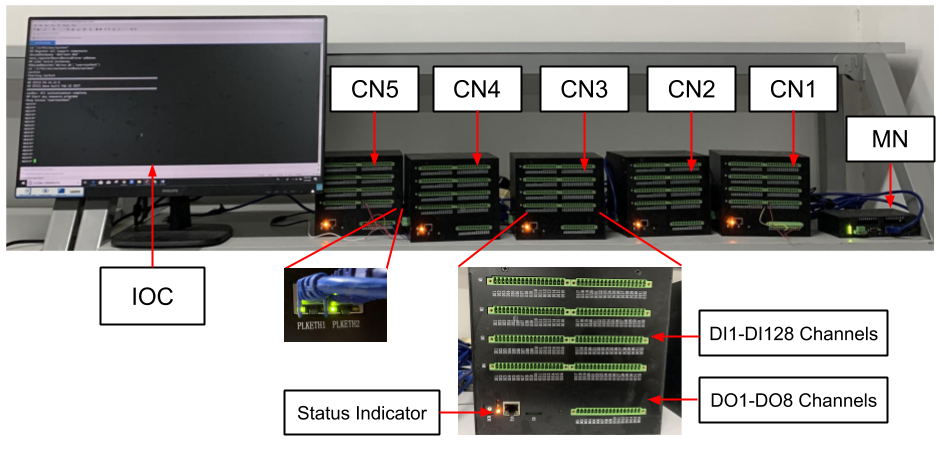
\includegraphics[width=\textwidth]{prototype-mn-fpga-photo.png}
  \caption{全站FPGA方案测试系统照片}
  \label{fig:prototype-mn-fpga-photo}
\end{figure}

\begin{figure}[htbp]
  \centering
  
\includegraphics[width=0.8\textwidth]{zynq-16di-interface.png}
  \caption{从站控制器DI接口}
  \label{fig:zynq-16di-interface}
\end{figure}

\begin{figure}[htbp]
  \centering
  
\includegraphics[width=0.8\textwidth]{zynq-16do-interface.png}
  \caption{从站控制器DO接口}
  \label{fig:zynq-16do-interface}
\end{figure}

\subsection{系统性能测试与分析}
\label{subsection:系统性能测试与分析}

\subsubsection{通信周期测试}
\label{subsection:系统通信周期测试}
全站FPGA方案系统的通信周期测试方式与主站PC方案相同,同样是使用ProfiShark 1G Ethernet Troubleshooter以太网诊断工具来测试系统在不同通信周期下的运行情况,从而确定系统最短通信周期。

\begin{figure}[!htb]
  \centering
  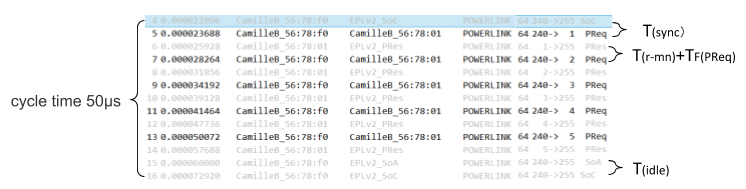
\includegraphics[width=\textwidth]{design2-cycle-time-test.png}
  \caption{测试系统POWERLINK数据帧抓取结果}
  \label{fig:design2-cycle-time-test}
\end{figure}

\begin{figure}[!htb]
  \centering
  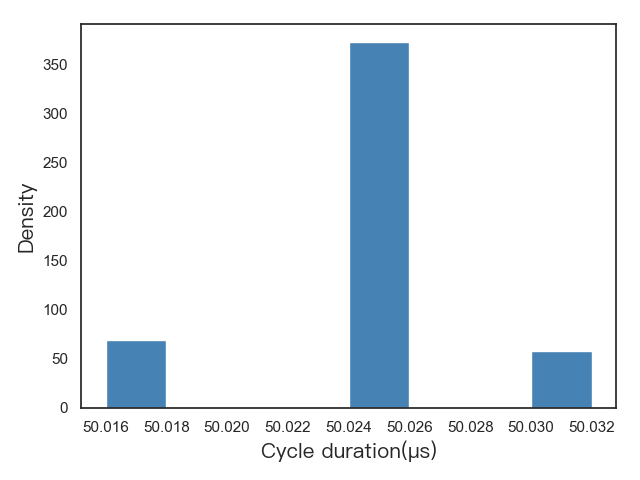
\includegraphics[width=\textwidth]{design2-cycle-time-density.png}
  \caption{测试系统POWERLINK通信周期概率密度分布}
  \label{fig:design2-cycle-time-density}
\end{figure}

全站FPGA方案的测试系统通信周期最快可配置为50$\mu$s,50$\mu$s通信周期下的通信过程如图~\ref{fig:design2-cycle-time-test}所示。我们抓取了超过20k个连续的POWERLINK数据帧,并将通信周期的概率密度分布绘制在图~\ref{fig:design2-cycle-time-density}中。该图显示大多数情况下的通信周期为50.024$\mu$s,少数情况为50.016$\mu$s和50.032$\mu$s,此结果是由基于Zynq的控制器和ProfiShark 1G以太网分析仪的125Mhz时钟频率引起的。通信周期周期的最大偏移仅为32$\mu$s,抖动非常小。

\subsubsection{响应时间测试}
\label{subsubsection:全FPGA方案的响应时间测试}
我们同样对全站FPGA方案进行了本地响应时间测试、全局响应时间测试和主站响应时间测试。

首先对从站控制器进行本地响应时间的测量,本地响应的过程如下:

1.系统从站的GPIO读取输入信号,并将输入值以二进制形式存储在FPGA的双口RAM中;

2.ARM通过32bit并行总线读取并处理RAM中的输入数据;

3.处理结果通过32bit并行总线写入相应的RAM中并通过GPIO输出信号。

选择测试系统中的5号从站控制器进行了本地响应时间测量,同样以输入和输出信号的上升沿时间差来表示本地响应时间。测试结果如图~\ref{fig:design2-local-response-time}所示,Ch2(青色线)代表5号从站控制器的输入信号;Ch3(红色线)代表5号从站控制器的输出信号,响应时间为5$\mu$s。这个时间延迟包括从站控制器输入/输出接口电路中的数字隔离器的延时和ARM读取处理数据的时间。由于ARM的时钟频率为125MHz,ARM读取处理数据的时间仅在$\mu$s量级,所以本地响应时间主要是由从站控制器的数字隔离器造成的,较之主站PC方案中的光耦合器,型号为ADuM1400的数字隔离器大大提高了信号传输速率。

\begin{figure}[!htb]
  \centering
  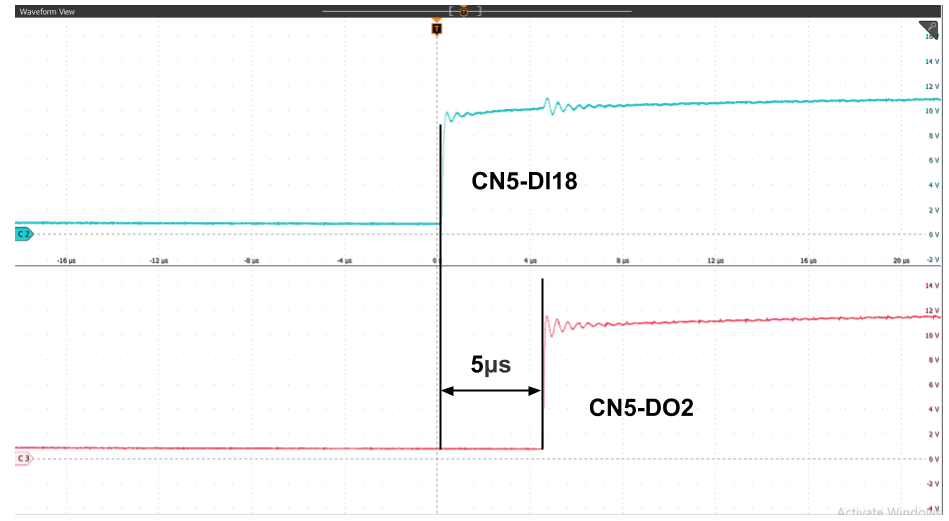
\includegraphics[width=\textwidth]{design2-local-response-time.png}
  \caption{本地响应时间测试结果}
  \label{fig:design2-local-response-time}
\end{figure}

\begin{figure}[!htb]
  \centering
  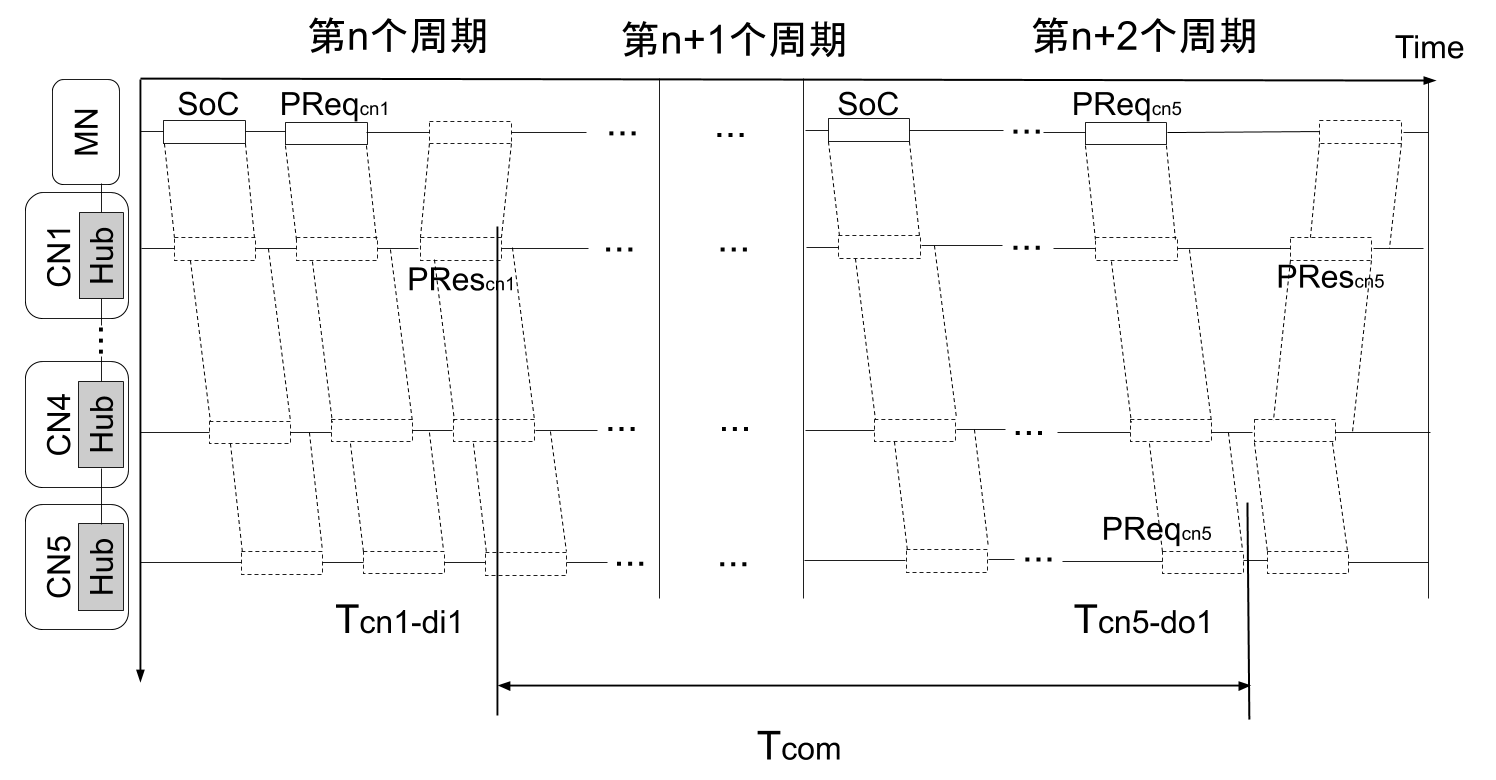
\includegraphics[width=\textwidth]{design2-response-process.png}
  \caption{系统全局响应过程}
  \label{fig:design2-response-process}
\end{figure}

全站FPGA方案的测试系统的全局响应时间($T_{global-response}$)由POWERLINK网络通信时间($T_{powerlink}$)和从站处理输入信号($T_{CN-process}$)的时间组成,见公式~\ref{equation17} 。

\begin{equation}
\label{equation17}
T_{global-response}=T_{powerlink}+T_{CN-process}
\end{equation}

在全局响应时间的测试中,我们设计了如图~\ref{fig:design2-response-process}所示的响应过程。在第n个周期,1号从站的输入信号通过PRes数据帧进入POWERLINK网络,$T_{cn1-di1}$为1号从站接收到输入信号的时刻,在第n+1个周期主站对该输入信号进行处理,处理结果在第n+2个周期通过PReq数据帧从5号从站输出,$T_{cn5-do1}$为5号从站输出信号的时刻。与主站PC方案通信过程不同的是,该响应过程需要经历三个连续周期,原因是主站对输入信号的处理时间为数$\mu$s,无法在本周期将处理结果传输出去。具体解释如下:在第n+2的周期开始的时候,主站发送SoC数据帧后产生同步中断信号,中断信号会触发应用层的同步回调函数“synCb( )”对“Sync Recv Buf”缓存区中的输入数据进行处理,这一过程的耗时为数$\mu$s,包括响应中断信号的时间、32bit并行总线读写的时间和数据处理的时间,所以处理结果只能在缓存区中等待下一个周期被发送出去。如图 ~\ref{fig:design2-response-process}所示,$T_{com}$是此过程的POWERLINK通信时间。根据POWERLINK通信顺序,5号从站是通信周期中的最后一个参与通信的,因此$T_{com}$也是该系统全局响应的最长通信时间。我们可以根据Wireshark抓包结果来计算第三个周期5号从站的PReq数据帧与第一个周期1号从站的PRes数据帧之间的时间差,从而得到$T_{com}$,大约为125$\mu$s。

从站处理输入信号的时间($T_{CN-process}$)包括数字隔离器的延时($T_{coupler}$)和输入信号在“Sync Send Buf”缓存区等待被发送的时间($T_{wait}$),见公式~\ref{equation18},其中数字隔离器的延时约为5$\mu$s。输入信号在进入从站控制器后并不会立刻进入POWERLINK网络,输入信号值需要在“Sync Send Buf”缓存区中等待回调函数“synCb()”读取后才可以传输到POWERLINK网络中,而“synCb()”需要SoC帧的触发才可以执行,所以输入信号的等待时间为信号进入系统到从站接收到SoC数据帧的时间差,最长为一个通信周期50$\mu$s。由公式~\ref{equation17}和~\ref{equation18}得,全局响应时间最长为180$\mu$s。

示波器测得的总响应时间如图~\ref{fig:design2-response-time-result}所示,Ch2(青色线)代表1号从站控制器的输入信号; Ch1(黑色线)代表5号从站控制器的输出信号,响应时间约为160$\mu$s。


\begin{equation}
\label{equation18}
T_{CN-process}=T_{coupler}+T_{wait}
\end{equation}

\begin{figure}[!htb]
  \centering
  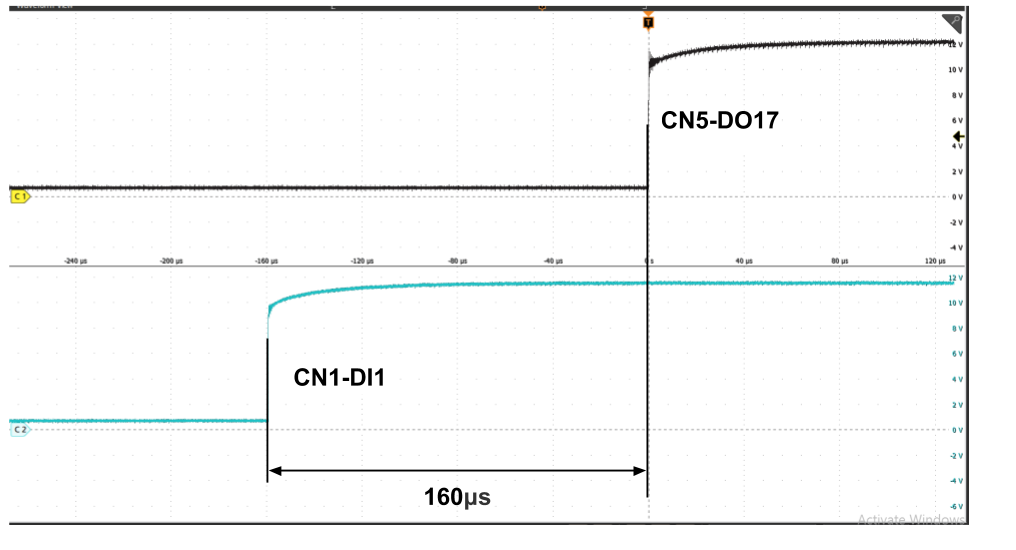
\includegraphics[width=\textwidth]{design2-response-time-result.png}
  \caption{全局响应时间测试结果}
  \label{fig:design2-response-time-result}
\end{figure}

全站FPGA方案的测试系统采用的基于Zynq的主站控制器。如图~\ref{fig:design2-cycle-time-test}所示,相邻PRes数据帧和PReq数据帧之间时间差为主站响应时间($T_{r-mn}$)和PReq数据帧的传输时间($T_{F(PReq)}$)之和。PReq数据帧长度为64Byte,采用千兆以太网传输,则$T_{F(PReq)}$为0.640$\mu$s。可得$T_{r-mn}$的平均值为1.737$\mu$s,基于Zynq控制器的响应时间平均值为1.717$\mu$s小于基于x86的pc16.168$\mu$s的响应时间,主站采用Zynq控制器来实现可以显著提升系统实时性能。

\subsubsection{测试小结}
本节对全站FPGA方案的测试系统进行了包括通信周期、系统响应时间和主站响应时间的性能测试,根据测试结果,总结如下:

(1) 全站FPGA方案的测试系统在5个节点情况下,可以在50$\mu$s通信周期下运行,系统全局响应时间为160$\mu$s。

(2)全站FPGA方案的测试系统主站采用Zynq控制器来实现,将主站响应时间缩短至1.737$\mu$s,较之主站PC方案中的pc主站,缩短了约14.4$\mu$s的响应时间。

(3) 全站FPGA方案的测试系统从站控制器的输入输出电路使用高速数字隔离器后,将本地响应时间缩短至5$\mu$s,较之主站PC方案的光耦合器,显著提高了信号传输的速率。

 (4) 全站FPGA方案的测试系统从站控制器使用4选1数据选择器,将每个从站控制器的DI通道扩展至128路。DO通道数扩展至16路。
 
 (5) 全站FPGA方案的测试系统在通信周期和主站响应时间等性能参数上优于主站PC方案,所以我们对基于全站FPGA方案开展进一步的研究。我们将采用第~\ref{section:理论计算POWERLINK通信周期}节和第~\ref{section:仿真模拟POWERLINK通信协议}节中发展的理论计算和仿真建模两种方法,对全站FPGA方案的POWERLINK系统通信周期进行估算。


\section{全站FPGA方案通信周期的理论计算}
\label{section:全站FPGA方案通信周期的理论计算}

本节根据第~\ref{section:理论计算POWERLINK通信周期}节中提出的POWERLINK通信周期的理论计算方法并结合全站FPGA方案测试系统的实测数据,推导出全站FPGA方案的POWERLINK系统的通信周期计算公式。

对于全站FPGA方案测试系统,主站和每个从站的用户数据均为2Byte时,PReq和PRes数据帧的大小均为64Byte,$T_{F(PReq)}$等于$T_{F(PRes)}$,根据第~\ref{section:理论计算POWERLINK通信周期}节中的从站通信间隙的相关公式~\ref{equation19}和~\ref{equation20}(与 2.3节中的相关公式类似), 我们可以得到公式~\ref{equation21}。该差值是个定值,即相邻从站时隙的差值为$2T_{c}+2T_{hub}$,表示从站时间间隙随着节点号的变大呈线性增长。

\begin{equation}
\label{equation19}
T_{rtd}^{i}=2iT_{c}+(2i-1)T_{hub}+T_{r-cn}
\end{equation}

\begin{equation}
\label{equation20}
T_{cn-slot}^{i}=T_{F(PReq)}^{i}+T_{F(PRes)}^{i}+T_{rtd}^{i}+T_{r-mn}
\end{equation}

\begin{equation}
\begin{split}
\label{equation21}
T_{cn-slot}^{i+1}-T_{cn-slot}^{i}&=T_{rtd}^{i+1}-T_{rtd}^{i}\\
&=2T_{c}+2T_{hub}
\end{split}
\end{equation}

如图~\ref{fig:test-theory-powerlink}所示,相邻两个PReq数据帧之间的时间差等于该从站时间间隙($T_{cn-slot}$),可以计算出每个从站的时间间隙,结果列于表~\ref{table:3.1}。

\begin{figure}[!htb]
	\centering
	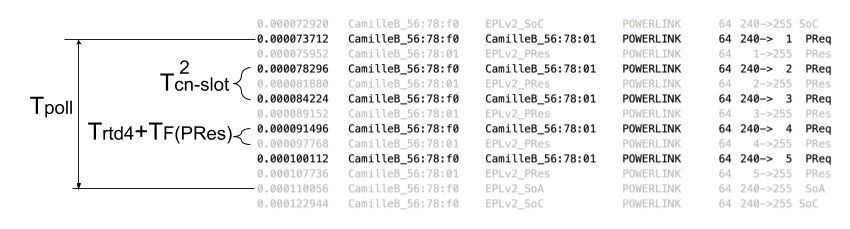
\includegraphics[width=\textwidth]{test-theory-powerlink.png}
	\caption{全站FPGA方案测试系统抓包结果}
	\label{fig:test-theory-powerlink}
\end{figure}

\begin{table}[hbtp]
  \centering
  \caption{从站时间间隙统计表:}
  \begin{tabular}{p{70 pt}p{70 pt}p{70 pt}p{70 pt}p{70 pt}}
    \toprule
    & Min & Max & Mean & Std.Dev\\
    \midrule
    $T_{cn-slot}^{1}$ & 4.560 & 4.584 & 4.572 & 0.0072\\
    $T_{cn-slot}^{2}$ & 5.900 & 5.940 & 5.910 & 0.0091\\
    $T_{cn-slot}^{3}$ & 7.250 & 7.300 & 7.260 & 0.0069\\
    $T_{cn-slot}^{4}$ & 8.660 & 8.590 & 8.607 & 0.0099\\
    $T_{cn-slot}^{5}$ & 9.910 & 9.980 & 9.929 & 0.0102\\
    \bottomrule
  \end{tabular}
  \\
  \footnotesize{所有数值均以$\upmu$s表示。}
  \label{table:3.1}
\end{table}


图~\ref{fig:fit-line}为从站平均时间间隙散点图,在图上添加了线性拟合趋势线,R平方值为1,表示拟合程度高,趋势线的可靠性高。拟合直线的斜率为1.341,等于$2T_{c}+2T_{hub}$。$T_{c}$为网线的延时,网线长度为2m,延时为(5ns/m),则$T_{hub}$为0.661$\mu$s。如图~\ref{fig:test-theory-powerlink}所示,相邻的PRes数据帧和PReq数据帧之间的时间差为$T_{rtd}^{i}$和$T_{F(PRes)}$之和,结合公式~\ref{equation19},可以计算得到$T_{r-cn}$的平均值为0.925$\mu$s。我们将一些重要通信参数的计算结果汇总列入表~\ref{table:3.2}中。

\begin{figure}[!htb]
  \centering
  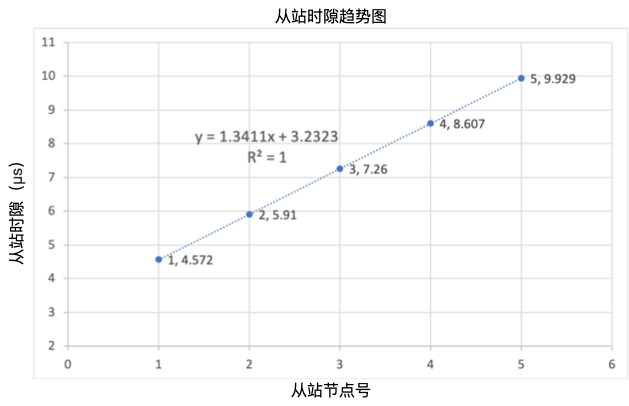
\includegraphics[width=\textwidth]{fit-line.png}
  \caption{从站时隙趋势图}
  \label{fig:fit-line}
\end{figure}

\begin{table}[hbt]
	\centering
	\caption{通信参数统计}
	\begin{tabular}{cccccc}
		\toprule
		主站响应时间($T_{r-mn}$) & 从站响应时间 ($T_{r-cn}$)& HUB延时 ($T_{hub}$)\\
		\midrule
		1.717μs & 0.925μs & 0.661μs\\
		\bottomrule
	\end{tabular}
	\label{table:3.2}
\end{table}


根据第~\ref{section:理论计算POWERLINK通信周期}节中的公式~\ref{equation22}、公式~\ref{equation23}和公示~\ref{equation24},并代入$T_{hub}$=0.661$\mu$s,$T_{r-cn}$=0.925$\mu$s,$T_{r-mn}$=1.717$\mu$s,我们可以推导出全站FPGA方案的等时同步阶段时长公式为~\ref{equation25}。

\begin{equation}
\label{equation22}
T_{poll}=T_{frames}+T_{net}
\end{equation}

\begin{equation}
\label{equation23}
T_{frames}=\sum_{i=1}^n(T_{F(PReq)}^{i}+T_{F(PRes)}^{i})
\end{equation}

\begin{equation}
\label{equation24}
T_{net}=\sum_{i=1}^nT_{rtd}^{i}+nT_{r-mn}
\end{equation}

\begin{equation}
\begin{split}
\label{equation25}
T_{poll}=&\sum_{i=1}^n(T_{F(PReq)}^{i}+T_{F(PRes)}^{i})+T_{net}^{line}\\
&=\sum_{i=1}^n(T_{F(PReq)}^{i}+T_{F(PRes)}^{i})+0.661n^{2}+2.642n
\end{split}
\end{equation}

对于全站FPGA方案系统,SoC帧的大小为64Byte,采用千兆以太网传输,$T_{F(SoC)}$仅为0.640$\mu$s,$T_{W}$为等待从站接收并处理SoC帧的时间,从站是基于Zynq的控制器,处理速度极快。由图~\ref{fig:design2-cycle-time-test}所示,同步过程($T_{sync}$)在1$\mu$s以内可以完成。考虑到空闲时间($T_{idle}$)为传输最大异步数据预留的时间,根据图~\ref{fig:design2-cycle-time-test}所示实测结果$T_{idle}$约为12.920$\mu$s,可得通信周期的公式~\ref{equation26},单位为$\mu$s。

\begin{equation}
\label{equation26}
\begin{split}
T_{cycle\_time}=&T_{F(SoC)}+T_{W}+\sum_{i=1}^n(T_{F(PReq)}^{i}+T_{F(PRes)}^{i})+n(n+1)T_{c}+n^2T_{hub}\\
& + n(T_{r-cn}+T_{r-mn})+T_{idle}\\
=&\sum_{i=1}^n(T_{F(PReq)}^{i}+T_{F(PRes)}^{i})+0.661n^{2}+2.642n+13.920
\end{split}
\end{equation}

\section{全站FPGA方案的仿真建模}
全站FPGA方案的仿真建模基于OMNet++网络模拟器展开,我们可以直接使用第~\ref{section:仿真模拟POWERLINK通信协议}建立了支持千兆POWERLINK通信的节点模型,然后结合实测参数对全站FPGA方案测试系统进行建模,将仿真结果和实测结果进行对比,来验证仿真建模方法的可行性,从而可将仿真建模方法应用于POWERLINK系统通信周期的估算。

首先对全站FPGA方案测试系统进行了建立了如图~\ref{fig:5node-model-omnet}所示的模型,节点数和拓扑结构均与测试系统保持一致,相邻节点之间通过2m长的网线相连,节点之间的通信基于千兆POWERLINK。对于测试系统中从站控制器的仿真建模,采用从站通信节点模块加上FPGA HUB模块来实现,两模块间传输延时设置为0$\mu$s。除此之外,为了准确地对测试系统进行仿真建模,采用测试系统中的实测参数对系统模型进行了配置,配置文件包括xdc\_cn\_std.xml和omnetpp.ini。xdc\_cn\_std.xml文件中配置了主站对各从站发送数据的大小(PReqActPayload)和各从站被分配的通信时隙(PResTimeout),其中各从站的通信时隙通过公式~\ref{equation19}和公式~\ref{equation20}得到,$T_{r-mn}$、$T_{r-cn}$、$T_{hub}$参数采用表~\ref{table:3.2}中的实测数据,具体配置如下:

\begin{figure}[!htb]
	\centering
	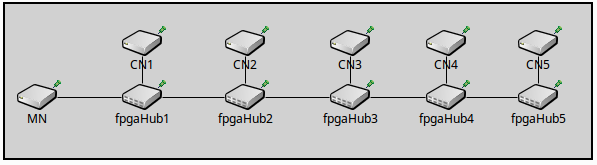
\includegraphics[width=0.9\textwidth]{5node-model-omnet.png}
	\caption{测试系统模型}
	\label{fig:5node-model-omnet}
\end{figure}

\begin{lstlisting}
<Nodes>
  <Node NodeId="1" PResTimeout="4617ns" PReqActPayload="2byte" />
  <Node NodeId="2" PResTimeout="5958ns" PReqActPayload="2byte" />
  <Node NodeId="3" PResTimeout="7299ns" PReqActPayload="2byte" />
  <Node NodeId="4" PResTimeout="8640ns" PReqActPayload="2byte" />
  <Node NodeId="5" PResTimeout="9981ns" PReqActPayload="2byte" />
</Nodes>
\end{lstlisting}

omnetpp.ini仿真配置文件包括了对系统通信周期、各从站节点号和响应数据大小、HUB延时的设定,具体内容如下:

\begin{lstlisting}
[Config EPLBase]
# 通信周期设置
**.MN.mnDll.cycleLenMean = 50us

# 各从站节点号和pres数据大小设定
**.CN1.cnDll.nodeId = 1
**.CN1.cnDll.presActPayload = 2
**.CN2.cnDll.nodeId = 2
**.CN2.cnDll.presActPayload = 2
**.CN3.cnDll.nodeId = 3
**.CN3.cnDll.presActPayload = 2
**.CN4.cnDll.nodeId = 4
**.CN4.cnDll.presActPayload = 2
**.CN5.cnDll.nodeId = 5
**.CN5.cnDll.presActPayload = 2

# FPGA HUB延时设定
**.hubDelayMean = 0.661us
\end{lstlisting}

模拟过程持续了大约3000个POWERLINK通信周期。因为同步阶段和同步阶段时长为定值,所以我们统计了等时同步阶段的时长,并将等时同步阶段概率密度分布绘制在图~\ref{fig:iso-time-density-5cn-model}中。该图表明大多数情况下的等时同步阶段时长为37.203$\mu$s,最大抖动不超过30ns。实测的等时同步阶段时长平均值为36.312$\mu$s,较之实测值,仿真建模方法对轮询阶段时长的计算误差在1$\mu$s以内。1$\mu$s误差对于50$\mu$s的通信周期来说影响非常小,所以仿真模拟方法可以准确的估算轮询阶段的时长。考虑到同步过程($T_{sync}$)在1$\mu$s以内可以完成以及12.920$\mu$s的空闲时间,通过仿真模拟得到的通信周期为51.120$\mu$s。

\begin{figure}[!htb]
  \centering
  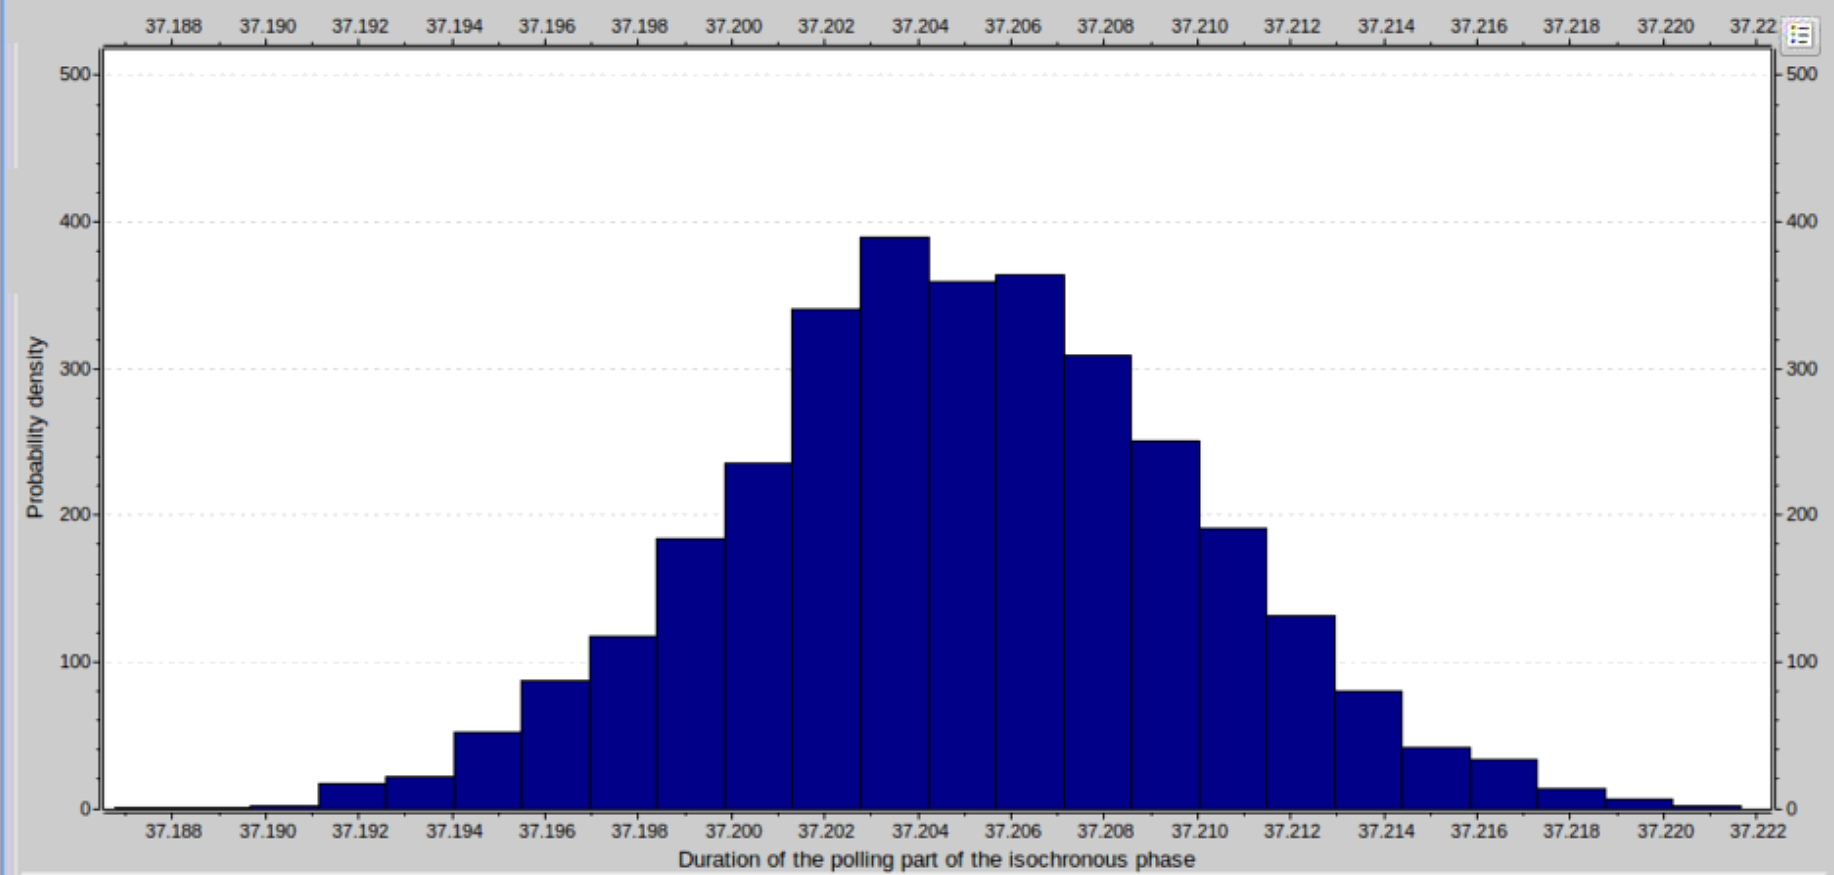
\includegraphics[width=\textwidth]{iso-time-density-5cn-model.png}
  \caption{测试系统模型轮询阶段的概率密度分布}
  \label{fig:iso-time-density-5cn-model}
\end{figure}







